\documentclass[convert={density=300,outext=.png}]{standalone}
\usepackage{tikz}
\usetikzlibrary{positioning}
\begin{document}
  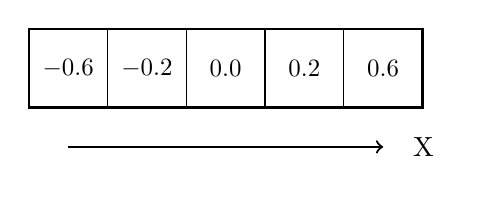
\begin{tikzpicture}[scale=1,every node/.style={minimum size=1cm},on grid]

    \fill[white,fill opacity=0.9] (0,0) rectangle (5,1);
    \draw[step=10mm, black] (0,0) grid (5,1); %defining grids
    \draw[black, thick] (0,0) rectangle (5,1); %marking borders

    \pgfkeys{/pgf/number format/.cd, fixed, zerofill, precision = 1}

    \foreach \x in {0,...,4} {
      \pgfmathsetmacro\rval{rand}
      \pgfmathparse{0.5+\x}
      \pgfmathresult \let\xpoint\pgfmathresult;
      \node[scale=0.9,thick] at (\xpoint,0.5)
      {$\pgfmathprintnumber{\rval}$};
    }

    \draw[thick,->] (0.5,-0.5) -- (4.5,-0.5) node[anchor=west] {X};
  \end{tikzpicture}
\end{document}
